\vspace{0.2cm}
\begin{figure}[!htb]
\begin{center}
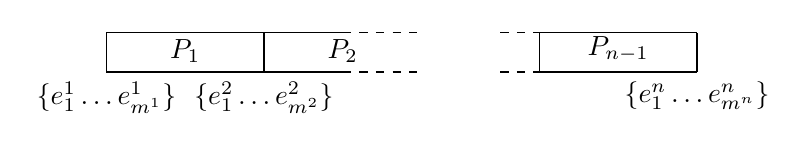
\begin{tikzpicture}

	\draw (0,0) -- (0,0.5);
	\draw (0,0) -- node[above]{$P_1$} (2,0);
	\draw (0,0.5) -- (2,0.5);
	\node[below] at (0,0) {$\{e_1^1\ldots e_{m^1}^1\}$};
	
	\draw (2,0) -- (2,0.5);
	\draw (2,0) -- node[above, xshift=0.5cm]{$P_2$} (3,0);
	\draw (2,0.5) -- (3,0.5);
	\node[below] at (2,0) {$\{e_1^2\ldots e_{m^2}^2\}$};
	\draw[dashed] (3,0) -- (4,0);
	\draw[dashed] (3,0.5) -- (4,0.5);
	
	
	\draw[dashed] (5,0) -- (5.5,0);
	\draw[dashed] (5,0.5) -- (5.5,0.5);
	\draw (5.5,0) -- (5.5,0.5);
	\draw (7.5,0) -- (7.5,0.5);
	\draw (5.5,0) -- node[above]{$P_{n-1}$} (7.5,0);
	\draw (5.5,0.5) -- (7.5,0.5);
	
	\node[below] at (7.5,0) {$\{e_1^n\ldots e_{m^n}^n\}$};
\end{tikzpicture}
\end{center}
\caption{Graphical representation of a the FunArray predicate.}\label{fig:funarraypredicate}
\end{figure}